%%%%%%%%%%%%%%%%%%%%%%%%%%%%%
% Standard header for working papers
%
% WPHeader.tex
%
%%%%%%%%%%%%%%%%%%%%%%%%%%%%%

\documentclass[11pt]{article}

%%%%%%%%%%%%%%%%%%%%
%% Include general header where common packages are defined
%%%%%%%%%%%%%%%%%%%%



%%%%%%%%%%%%%%%%%%%%%%%%%%
%% Packages
%%%%%%%%%%%%%%%%%%%%%%%%%%


% general packages without options
\usepackage{amsmath,amssymb,bbm}

% graphics
\usepackage{graphicx}

% text formatting
\usepackage[document]{ragged2e}
\usepackage{pagecolor,color}




\usepackage[utf8]{inputenc}
\usepackage[T1]{fontenc}
%\usepackage[francais]{babel}



% for framed figures or texts
\usepackage{mdframed}



%%%%%%%%%%%%%%%%%%%%
%% Idem general commands
%%%%%%%%%%%%%%%%%%%%
%% Commands

\newcommand{\noun}[1]{\textsc{#1}}


%% Math

% Operators
\DeclareMathOperator{\Cov}{Cov}
\DeclareMathOperator{\Var}{Var}
\DeclareMathOperator{\E}{\mathbb{E}}
\DeclareMathOperator{\Proba}{\mathbb{P}}

\newcommand{\Covb}[2]{\ensuremath{\Cov\!\left[#1,#2\right]}}
\newcommand{\Eb}[1]{\ensuremath{\E\!\left[#1\right]}}
\newcommand{\Pb}[1]{\ensuremath{\Proba\!\left[#1\right]}}
\newcommand{\Varb}[1]{\ensuremath{\Var\!\left[#1\right]}}

% norm
\newcommand{\norm}[1]{\| #1 \|}


%% graphics

% renew graphics command for relative path providment only ?
%\renewcommand{\includegraphics[]{}}



% geometry
\usepackage[margin=2cm]{geometry}

\usepackage{float}

% layout : use fancyhdr package
\usepackage{fancyhdr}
\pagestyle{fancy}

\makeatletter

\renewcommand{\headrulewidth}{0.4pt}
\renewcommand{\footrulewidth}{0.4pt}
\fancyhead[RO,RE]{15-17/03/2017}
\fancyhead[LO,LE]{TP1}
\fancyfoot[RO,RE] {\thepage}
\fancyfoot[LO,LE] {L1 54BEG3GO - S2 2017}
\fancyfoot[CO,CE] {}


\fancypagestyle{firststyle}
{
   \fancyhf{}
   \fancyhead[RO,RE]{TP1 - 15-17/03/2017}
   \fancyhead[LO,LE]{L1 54BEG3GO - S2 2017}
}


%\renewcommand{\abstractname}{Objectifs du TD}

\renewcommand{\figurename}{\textbf{Document}}


\makeatother


%%%%%%%%%%%%%%%%%%%%%
%% Begin doc
%%%%%%%%%%%%%%%%%%%%%

\begin{document}









\title{\textbf{Statistiques et Cartographie - TP1}}

\date{}


\maketitle

\justify

\thispagestyle{firststyle}


\textit{\textbf{Consignes : }Le tableau de données et de travail }\texttt{StatCarto{\_}TP1.xlsx}\textit{ est à télécharger sur Moodle ; vous ne serez pas notés sur le contenu final du fichier mais sur votre copie uniquement, sur laquelle il faudra bien noter tous les résultats demandés.}


\bigskip


\section*{Exercice : Connaissance des Risques d'Inondation}

Ce travail se base sur les données d'enquête que vous avez saisies lors du TD2. On propose de s'intéresser à la connaissance du risque d'inondation par les sondés. Sur 185 grilles saisies, 182 sont exploitables en terme de localisation précise de la commune des sondés.


\paragraph{Contexte (3pts)}

% blabla contexte, quanti quali etc

$\rightarrow$ \textit{Discutez de problématiques possibles à partir des données que vous avez recueillies et saisies ; quels peuvent être les apports et limitations d'une approche quantitative, et comment peut-elle être complémentaire d'une approche qualitative ? Pensez vous que la distinction quantitatif-qualitatif soit pertinente en géographie contemporaine ?}




\paragraph{Données (2pts)}

% carte de loc, commentaire

$\rightarrow$ \textit{Commentez la distribution spatiale des lieux de résidence des sondés (Document 1). La quantité de 182 réponses vous semble-t-elle suffisante pour tirer des conclusions statistiques robustes ? Pourquoi ?}

%Il faut ainsi garder à l'esprit la limitation des statistiques sur de faibles échantillons, la majorité des méthodes vues en cours étant valables





\paragraph{Statistiques générales (5pts)}

L'onglet \texttt{Donnees} donne l'ensemble des scores donnant le niveau de connaissance du phénomène de crue (nombre entier entre 1 et 5).

$\rightarrow$ \textit{Tracez le diagramme de distribution du niveau de connaissance (à reproduire sur votre copie) ; calculez moyenne et écart-type}\footnote{la formule vue en cours est implémentée par la fonction \texttt{ECARTTYPE} d'Excel\textregistered, tandis que la fonction \texttt{ECARTTYPEP} implémente l'estimateur non-biaisé de la variance. Le biais intrinsèque à l'estimateur standard est dû à l'utilisation de la moyenne estimée au sein de l'estimateur de variance. Il tend vers 0 quand la taille de l'échantillon tend vers l'infini. Dans notre cas, il est de l'ordre relatif du millième, vous pouvez utiliser la fonction de votre choix sans impact significatif sur le résultat.}\textit{ de l'échantillon. Commentez la forme de la distribution et les valeurs obtenues.}


\paragraph{Rôle de la proximité et de l'accessibilité aux zones inondables (5pts)}

On cherche à savoir si la distance du domicile à une zone inondable influence la connaissance des risques, autrement dit si les populations les plus concernées sont aussi informées. On suppose que l'ignorance est distribuée uniformément dans les populations et donc dans l'espace, et on s'intéresse aux réponses satisfaisant un certain niveau de connaissance (au moins 3). On a calculé pour chaque commune la distance à une zone inondable, et classé les réponses dans deux classes pour simplifier (``proche'', si la distance est inférieure à 2km, ``lointain'' si elle est supérieure), dans l'onglet \texttt{Distance}\footnote{Le document 3 cartographie les distances par commune.}.

\medskip

$\rightarrow$ \textit{Calculez moyenne et écart-type pour chacune des classes (aide : utiliser la fonction ``trier'' pour ordonner par classe). Proposez une interprétation sur l'effet de la distance.}


La distance brute ne prend pas en compte l'intensité des inondations potentielles (voir surfaces inondables en document 2). Pour cela, on définit une mesure ``d'accessibilité aux zones inondables''\footnote{qui correspond à la moyenne des surfaces des zones inondables pondérées par la distance à la commune, donnée pour la commune $i$, avec $A_j$ surfaces des zones inondables, $Z_i = \sum_j A_j\cdot \exp\left(- d_{ij}/d_0 \right)$ avec ici $d_0=5km$. Elle est également cartographiée en document 3.} qu'il faut interpréter comme une quantité d'inondation potentielle dans un voisinage géographique de la commune. L'onglet \texttt{Accessibilite} donne ces valeurs et une classification simplifiée (``haute'' et ``basse'').

\medskip

$\rightarrow$ \textit{De même, calculez moyenne et écart-type pour chaque classe. Interprétez et comparez aux résultats pour la distance.}


\paragraph{Point de vue cartographique (2pts)}

$\rightarrow$ \textit{Commentez la synthèse cartographique du niveau de connaissance en document 2 ; est-il possible de tirer de conclusions générales à partir de la carte uniquement ? Dans quelle mesure la cartographie et l'analyse statistique sont-elles complémentaires ?}




% à quoi exactement correspondent les zones inondables ?



\paragraph{Autres variables (2pts)}

$\rightarrow$ \textit{En correspondance à des problématiques proposées en première question, discutez d'autres variables ou aspects\footnote{Qui peuvent être dans le questionnaire initial ou non ; souvent un premier questionnaire pilote est administré et le questionnaire est modifié selon les réponses obtenues, pour adapter ou préciser des points.} qui seraient pertinents à prendre en compte.}


\paragraph{Données Synthétiques (1pts)}

$\rightarrow$ \textit{Discutez de l'intérêt d'extrapoler des données manquantes (communes sans répondant) ou de simuler des données synthétiques (réponses ayant la même structure statistique) à partir du jeu de données disponibles.}



\begin{figure}
\centering
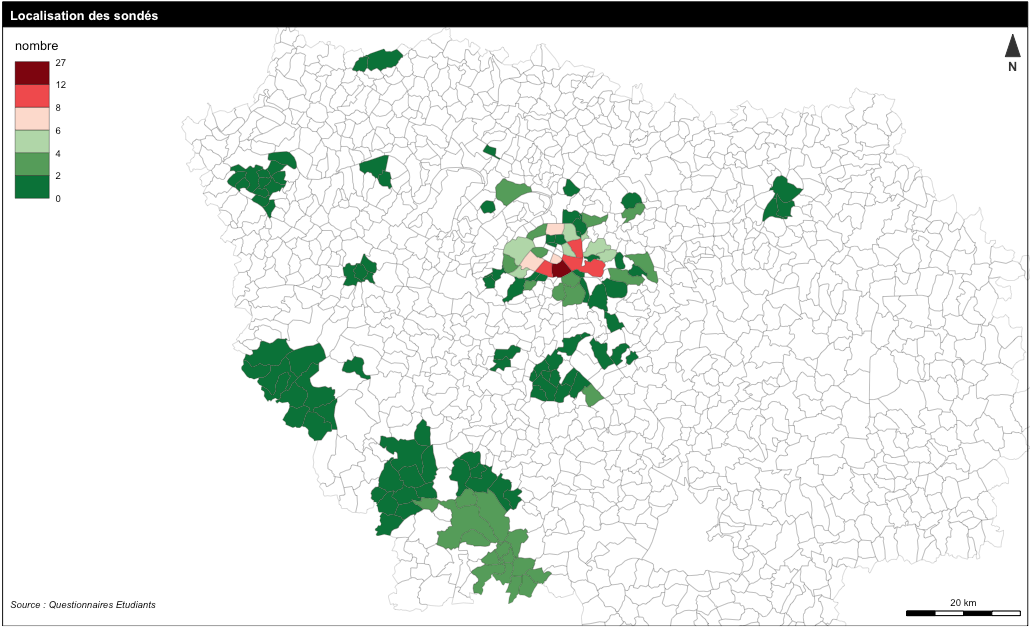
\includegraphics[width=\textwidth,height=0.45\textheight]{maps/count2}
\caption{Nombre de réponses au sondage par communes (code postal).}
\end{figure}


\begin{figure}
\centering
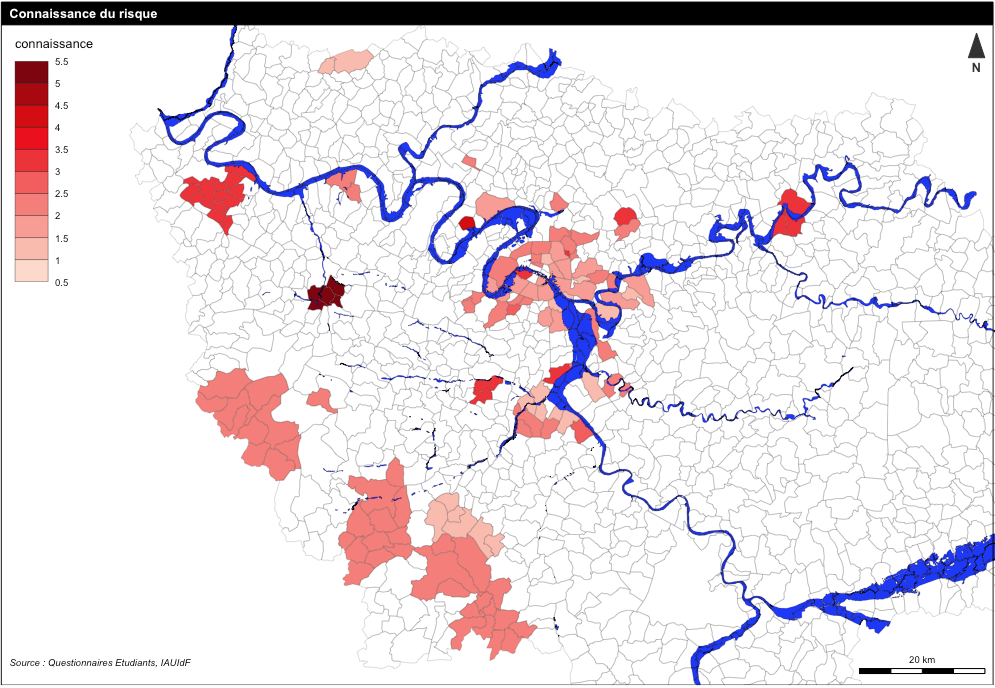
\includegraphics[width=\textwidth,height=0.43\textheight]{maps/knowledge_moreclass}
\caption{Niveau moyen de connaissance du risque agrégé par code postal ; zones inondables (Plus Hautes Eaux Connues).}
\end{figure}



\begin{figure}
\centering
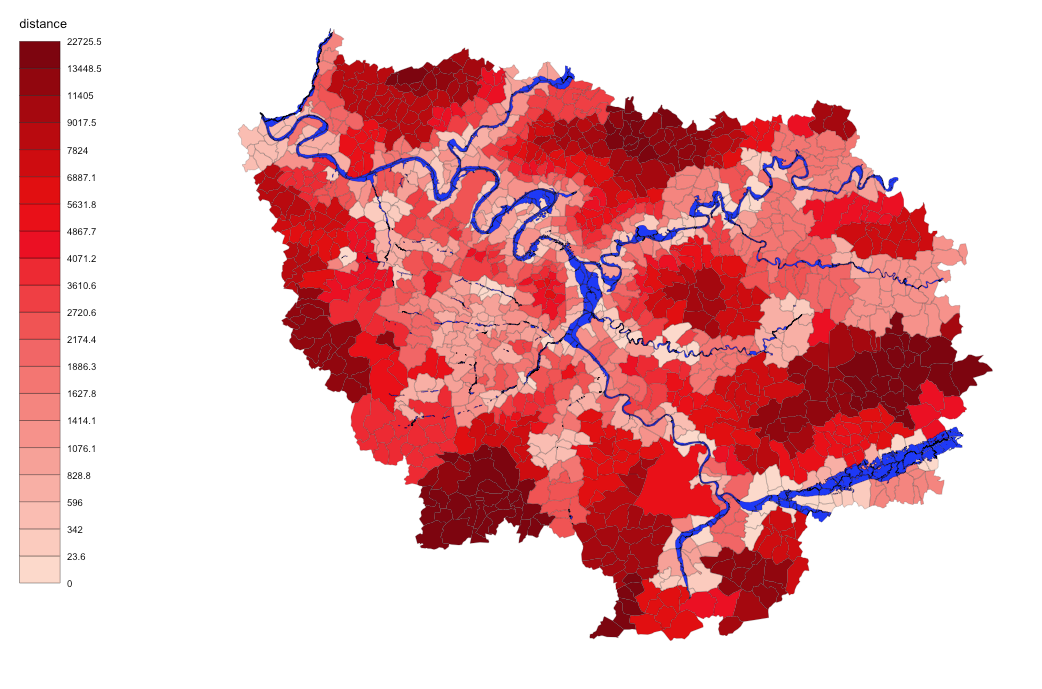
\includegraphics[width=0.48\textwidth]{maps/distance2}
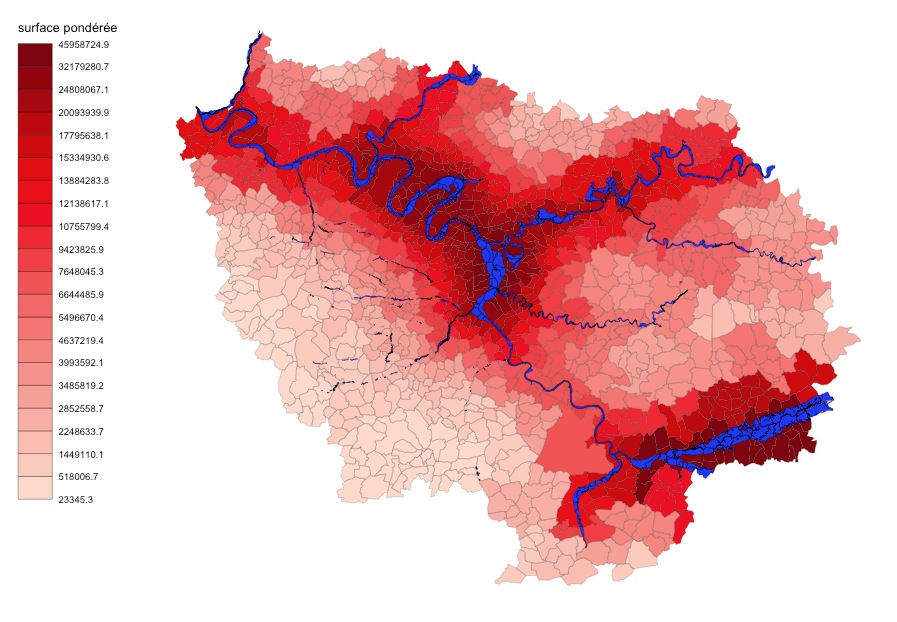
\includegraphics[width=0.48\textwidth]{maps/surfponderee}
\caption{(Gauche) Distance des communes aux zones inondables ; (Droite) Surface accessible de zone inondable.}
\end{figure}





%\bigskip
%\bigskip
%
%\strut\hfill$\star$\hspace{1.2cm}$\star$\hfill\strut\vspace{0.1cm}\\
%
%\strut\hfill$\star$\hfill\strut\par





\section*{Exercice Facultatif}


\textit{\textbf{Consigne : }Exercice à traiter si vous avez fini le premier largement en avance et facilement.}

\bigskip

La question de la ``robustesse statistique'' d'une estimation, par exemple dans notre cas d'une moyenne ou d'un écart-type, est essentielle pour la validation des interprétations qu'on peut en tirer. On se propose d'illustrer cette notion dans un cas simple, sur un jeu de données synthétiques.












\end{document}